In this subsection we give an overview for the SmartMPSDockingRoboCup component, regarding the different states and tasks. Currently there are two components, an old and a new version. Both will be discussed and compared to each other. In the end we will provide an introduction into the mapping aspect of this component and how the calculation of the orientation of MPS works.

\subsubsection{Overview}

\begin{figure}[h]
\centering
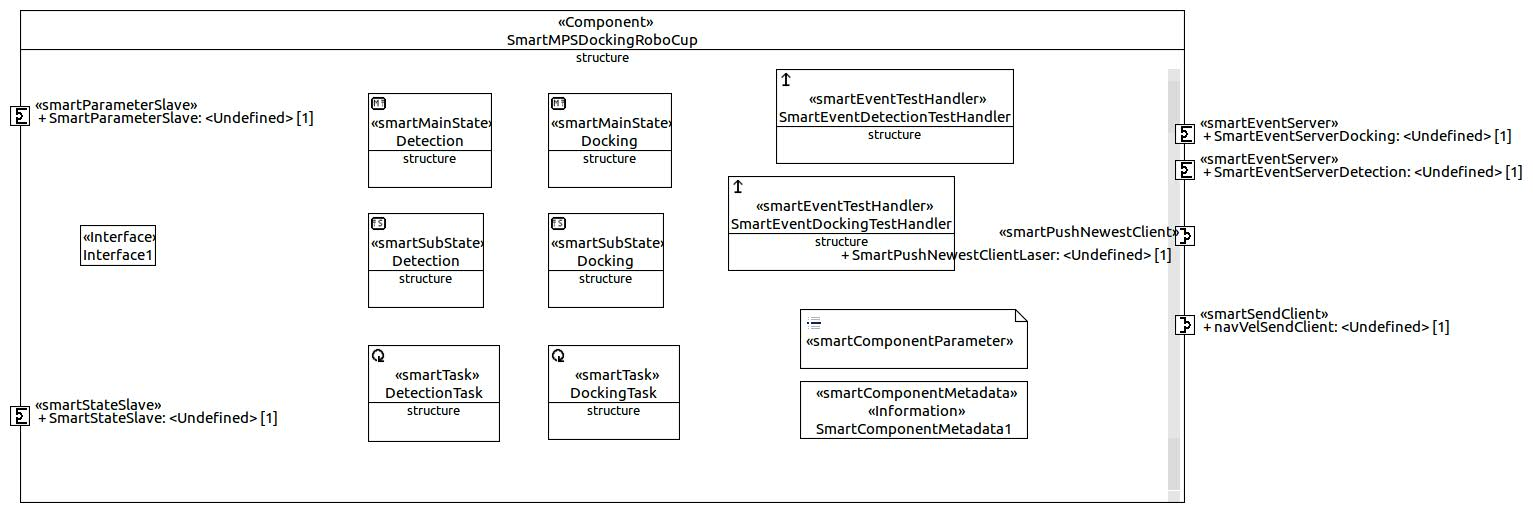
\includegraphics[scale=0.4]{pic/SmartMPSDockingRoboCup.JPG}
\caption{Model of MPS Detection/Docking Component}
\label{fig:i_overview}
\end{figure}

The SmartMPSDockingRoboCup component has two main tasks:

\begin{enumerate}
\item Detection of MPS
\item Docking to MPS
\end{enumerate}

\paragraph{Detection}
The detection of MPS is realized in the DetectionTask of the component. This task has a corresponding State and Substate which is called Detection. The Task is reliant on the SmartPushNewestClientLaser. This port is connected to the component which abstracts the laser range finder and provides the latest laser scan as a point cloud. Based on this information the DetectionTasks determines whether lines could correspond to a MPS. \\


\paragraph{Docking}
The docking to an MPS is implemented in the DockingTask, which has a State and Substate called Docking (like the DetectionTask). Currently the DockingTask is based on the MPS found with the DetectionTask. These serve as a direct input for the DockingTask which utilizes the NavVelSendClient to drive the robot to the nearest MPS found.

\subsubsection{CommObjects}
The component has two ports which propagate information to other components. These ports are SmartEventServerDocking which sends messages of the type CommStationDockingEventState and the 
SmartEventServerDetection which sends messages of the type CommStationDockingEventState. Connecting another component to these ports will yield the information described below. 
\\
With regards to event results and state both DetectionTask and DockingTask work in a similar fashion. Each task has a distinct EventState:
\begin{itemize}
\item CommStationDetectionEventState
\item CommStationDockingEventState
\end{itemize}
The content of the EventState is the an instantiation of an EventResult:
\begin{itemize}
\item CommStationDetectionEventResult
\item CommStationDockingEventResult
\end{itemize}
This EventResult is the resulting information which is computed by the execution of a Task. However the content of the EventResults is different for each task. This is elaborated in the following paragraphs.

\paragraph{Detection}
The CommStationDetectionEventResult contains

\begin{enumerate}
\item MPSStationDetectionResult
\item CommMPSStationData (as a vector)
\end{enumerate}

The MPSStationDetectionResult is an enum which provides general information whether a MPS was found (MPS\_FOUND) or not (NO\_MPS\_FOUND).
If no MPS is found by the DetectionTask, the CommMPSStationData vector is empty, however if MPS are determined, there is a vector of CommMPSStationData containing the following information:

\begin{itemize}
\item orientation1 -> radial orientation corresponding to first docking point
\item orientation2 -> radial orientation corresponding to second docking point
\item centerX -> X coordinate of the MPS center point
\item centerY -> Y coordinate of the MPS center point
\item dockingPosX1 -> X coordinate of the first docking point
\item dockingPosX2 -> X coordinate of the second docking point
\item dockingPosY1 -> Y coordinate of the first docking point
\item dockingPosY2 -> Y coordinate of the second docking point
\item zone -> Zone of the Robocup map where the MPS resides
\end{itemize}

In general the docking points are points perpendicular to the MPS station with a distance that is adjusted in the components parameters (default 1m). There are two points and orientations for the front and the back of the MPS. However the first docking point is always the point, which is nearest to the Robotino. The orientation corresponds to the orientation used by the mapping and base components of the Robotino, therefore rotating the Robotino to an orientation results in the Robotino to face the front or the back of the MPS.
	
\paragraph{Docking}

CommObject CommStationDockingEventResult 
new\_state  EnumRef ( StationDockingState )
		
Enum StationDockingState 
DOCKING\_DONE
DOCKING\_NO\_STATION
DOCKING\_UNKNOWN
	
\subsubsection{Previous State}
DeployMPSDocking NEW
DeployJaegerTest OLD

\subsubsection{Current State}

\subsubsection{Mapping}


